\section{Climate Calculations}\label{climate-calculations}

The location of the facility under analysis is critical for the determination of energy consumption, heating/cooling loads, daylighting potential, and a host of other calculations. In EnergyPlus, both external (i.e, weather files supplied from others) and internal (i.e., solar position, design day temperature/humidity/solar profiles) data is used during simulations.

The ``Site:Location'' input object includes parameters (Latitude, Longitude, Elevation, Timezone) that allow EnergyPlus to calculate the solar position (using Latitude, Longitude and Timezone) for any day of the year as well as supply the standard barometric pressure (using elevation). Solar position modeling is discussed in more detail in both the Sky Radiance and Shading Calculation sections that directly follow this section.

Weather files have hourly or sub-hourly data for each of the critical elements needed during the calculations (i.e., Dry-Bulb Temperature, Dew-Point Temperature, Relative Humidity, Barometric Pressure, Direct Normal Radiation, Diffuse Horizontal Radiation, Total \& Opaque Sky Cover, Wind Direction, Wind Speed) as well as some auxiliary data such as Rain or Snow that assist in certain calculational aspects. Weather file excerpts such as might be used in sizing calculations also have this breadth of data. The input object ``SizingPeriod:DesignDay'' describes design days (meant to mimic ASHRAE design conditions but in a whole day profile) using certain characteristics for the day and then EnergyPlus supplies the remaining portions to complete outdoor conditions needed for program execution. SizingPeriod:DesignDay are perhaps the best objects for sizing equipment as the ASHRAE specified design conditions can be input AND weather files may or may not have the conditions necessary to size equipment properly.

Two other objects, however, can be used at times: SizingPeriod:WeatherFileDays and SizingPeriod:WeatherFileConditionType.~ With the first of these, one specifies a set of weather file days similar to a RunPeriod (but will be used for the Sizing calculations). In the second, the extreme or typical conditions that are calculated for the weather file during processing can be used by name.~ Of course, either of these can be used as a measure of usage over small periods.

The ASHRAE Handbook of Fundamentals describes their criteria in creating design condition synopses. ``Design data based on dry-bulb temperature represent peak occurrences of the sensible component of ambient outdoor conditions. Design values based on wet-bulb temperature are related to the enthalpy of the outdoor air. Conditions based on dewpoint relate to the peaks of the humidity ratio. The designer, engineer, or other user must decide which set(s) of conditions and probability of occurrence apply to the design situation under consideration.''

\subsection{EnergyPlus Design Day Temperature Calculations}\label{energyplus-design-day-temperature-calculations}

In EnergyPlus, the typical design day input includes a ``high'' and a ``low'' dry-bulb temperature for the day. As these two temperatures are insufficient to represent a full 24 hour period, the program uses a ``range multiplier'' profile to represent the full day's temperatures:

\begin{figure}[hbtp] % fig 36
\centering
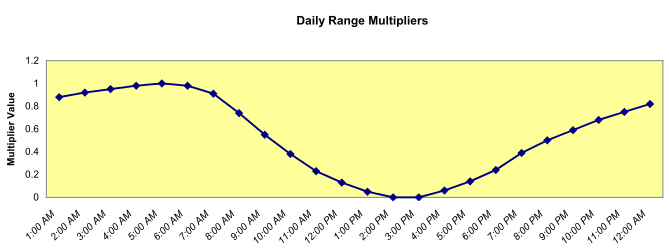
\includegraphics[width=0.9\textwidth, height=0.9\textheight, keepaspectratio=true]{media/image563.svg.png}
\caption{Default Daily Temperature Range Profile \protect \label{fig:default-daily-temperature-range-profile}}
\end{figure}

The multipliers are taken from the ASHRAE 2009 HOF, Table \# 6, p.~14.11.. More explicitly, EnergyPlus creates an air temperature for each timestep by using the entered maximum dry-bulb temperature in conjunction with the entered daily range and the above multiplier values. The actual equation used is shown below:

\begin{equation}
{T_{current}} = {T_{Max}} - {T_{range}}\cdot {T_{Multiplier}}
\end{equation}

where

T\(_{current}\) = Air temperature of current Hour of Day

T\(_{Max}\) = User supplied Max Dry-bulb Temperature

T\(_{range}\) = User supplied Daily Temperature Range

T\(_{Multiplier}\) = Range multiplier as shown on the above graph

The range multiplier values represent typical conditions of diurnal temperatures (i.e.~the low temperature for the day occurring about 5:00 AM and the maximum temperature for the day occurring about 3:00 PM.~ Note that EnergyPlus does not shift the profile based on the time of solar noon as is optionally allowed by ASHRAE procedures.

ASHRAE research indicates that dry-bulb and wet-bulb temperatures typically follow the same profile, so EnergyPlus can use the default daily temperature profile to generate humidity conditions based on maximum and range of wet-bulb temperature.

Since this default temperature profile may not be applicable to all locations, the user can give a different profile as part of the design day definition.

\subsection{Sky Radiation Modeling}\label{sky-radiation-modeling}

EnergyPlus calculates the Horizontal Infrared Radiation Intensity ($IR_H$), if it is missing in the weather file or for design days, from the Dry Bulb Temperature, Dewpoint Temperature or Partial Pressure of Water Vapor, and Opaque Cloud Cover as described below. Regardless of whether or not $IR_H$ is present in the weather file, it can be specified in the \textbf{WeatherProperty:SkyTemperature} object to ignore the reported value of $IR_H$ and instead calculate it from the specified sky emissivity model as described below.

$IR_H$ is defined as the rate of infrared radiation emitted from the sky falling on a horizontal upward-facing surface, in \si{\watt\per\m\squared}.

\begin{equation}
IR_H = \sigma T_{sky}^4
\end{equation}

\noindent where:
\newline

$\sigma$ = Stefan-Boltzmann constant = \SI{5.6697e-8}{\watt\per\meter\squared\per\kelvin\tothe{4}}

$T_{sky}$ = Effective mean sky temperature, or sky radiative temperature, \si{\kelvin}.
\newline

Over the years authors have proposed a fictitious quantity called the Sky Emissivity ($\epsilon_{sky}$) such that the following energy balance is satisfied:

\begin{equation}
IR_H = \epsilon_{sky} \cdot \sigma \cdot T_{db}^4
\end{equation}

$\epsilon_{sky}$ = sky emissivity

$T_{db}$ = drybulb temperature, \si{\kelvin}
\newline

Four correlations for $\epsilon_{sky}$ under clear-sky conditions, proposed by four sets of authors, are available in EnergyPlus. The default correlation is from Clark \& Allen (1978):

\begin{table}[hbtp]
\centering
\begin{tabular}{cl}
\textbf{Author}   & $\epsilon_{sky, clear}$ \\ \\
Clark \& Allen    & $= 0.787 + 0.764 \ln\left(T_{dp}/273\right)$ \\ \\
Martin \& Berdahl & $= 0.758 + 0.521 \left(T_{dp}/100\right) + 0.625  \left(T_{dp} / 100\right)^2$ \\ \\
Brunt             & $= 0.618 + 0.056 \left(P_{wv}\right)^{0.5}$ \\ \\
Idso              & $= 0.685 + 3.2\times10^{-5} \left(P_{wv}\right) e^{1699/T_{db}} $
\end{tabular}
\end{table}

\noindent where:
\newline

$\epsilon_{sky, clear}$ = $\epsilon_{sky}$ under clear-sky conditions
\newline

$T_{dp}$ = dewpoint temperature, in \si{\kelvin} for Clark \& Allen, in \si{\celsius} for Martin \& Berdahl
\newline

$P_{wv}$ = partial pressure of water vapor, in \si{\hecto\pascal}
\newline

The clear sky emissivity is modified for partially-cloudy conditions using the correlation from Walton (1983) which uses the opaque cloud cover fraction:

\begin{equation}
\epsilon_{sky} = \epsilon_{sky, clear} \left(1 + 0.0224  N - 0.0035  N^2 + 0.00028  N^3\right)
\end{equation}

\noindent where:
\newline

$N$ = opaque sky cover, in tenths.
\newline

\noindent Example:
\newline

Clear sky ($N=0$), $T_{db} = 20 + 273.15 = \SI{293.15}{\kelvin}$, $T_{dp} = 10 + 273.15 = \SI{283.15}{\kelvin}$
\newline

$\epsilon_{sky} = \left(0.787 + 0.764  \ln\left(283.15/273\right)\right)  \left(1 + 0.0224  N - 0.0035  N^2 + 0.00028  N^3 \right) = 0.815$
\newline

$IR_H = 0.815 \times 5.6697 \times 10^{-8} \times 293.15^{4} = \SI{341.2}{\watt\per\meter\squared}$
\newline

References for these calculations are contained in the references section at the end of this list of fields. (Walton, 1983) (Clark \& Allen, 1978), (Li et al, 2017).

\subsection{EnergyPlus Sky Temperature Calculation}\label{energyplus-sky-temperature-calculation}

By default the Sky Temperature ($T_{sky}$) is calculated from the Horizontal Infrared Radiation Intensity ($IR_H$):

\begin{equation}
T_{sky} = \left(IR_H / \sigma\right)^{0.25} - 273.15
\end{equation}

\noindent where:
\newline

$T_{sky}$ = Effective mean sky temperature, or sky radiative temperature, in \si{\celsius}.
\newline

$IR_H$ = rate of infrared radiation emitted from the sky falling on a horizontal upward-facing surface, in \si{\watt\per\meter\squared}.
\newline

$\sigma$ = Stefan-Boltzmann constant = \SI{5.6697e-8}{\watt\per\meter\squared\per\kelvin\tothe{4}}
\newline

(Note: T\{\si{\celsius}\} = T\{\si{\kelvin}\} - 273.15)
\newline

The Sky Temperature can also be set by the user from several options using the~\textbf{WeatherProperty:SkyTemperature} object.

\subsection{EnergyPlus Design Day Solar Radiation Calculations}\label{energyplus-design-day-solar-radiation-calculations}

Similarly, calculating solar irradiance (solar modeling) is one of the important effects to be accomplished. Several solar models exist with varying complexity.

\subsubsection{ASHRAE Clear Sky Solar Model}\label{ashrae-clear-sky-solar-model}

The default model used is the ASHRAE Clear Sky model. The ASHRAE clear sky model described in ASHRAE HOF 2005 Chapter 31 can be used to estimate hourly clear-day solar radiation for any month of the year in U.S. or similar temperate climates in the northern hemisphere. EnergyPlus calculations extend the clear sky application to both northern and southern hemispheres.~ Note that the Clear Sky model has been updated in the ASHRAE HOF 2009 (see ASHRAE Revised Clear Sky Model below).

At the earth's surface on a clear day, direct normal irradiation is represented by

\begin{equation}
Direct\;Normal\;Irradiation = \frac{A}{exp\left( \frac{B}{\sin \beta } \right)}
\label{eq:DirectNormalIrradiation}
\end{equation}

where

\emph{A} = apparent solar irradiation at air mass m = 0 (Table~\ref{table:extraterrestrial-solar-irradiance-and-related})

B = atmospheric extinction coefficient Table~\ref{table:extraterrestrial-solar-irradiance-and-related})

Values of A and B vary during the year because of seasonal changes in the dust and water vapor content of the atmosphere and because of the changing earth-sun distance. Equation~\ref{eq:DirectNormalIrradiation} does not give the maximum value of direct normal irradiation that can occur in each month but yields values that are representative of conditions on cloudless days for a relatively dry and clear atmosphere. For very clear atmospheres, direct normal irradiation can be 15\% higher than indicated by Equation~\ref{eq:DirectNormalIrradiation}, using values of A and B in Table~\ref{table:extraterrestrial-solar-irradiance-and-related} below.

% table 20
\begin{longtable}[c]{p{0.75in}p{0.75in}p{0.75in}p{0.75in}p{0.75in}p{0.75in}p{0.75in}}
\caption{Extraterrestrial Solar Irradiance and Related Data Note: Data are for 21st day of each month during the base year of 1964. \label{table:extraterrestrial-solar-irradiance-and-related}}\\
\toprule
~ & I\(_{o}\)\{W/m\(^{2}\)\} & Equation of Time \{minutes\} & Declination \{degrees\} & A \{W/m\(^{2}\)\} & B \{\} & C \{\} \tabularnewline
\midrule
\endfirsthead

\caption[]{Extraterrestrial Solar Irradiance and Related Data Note: Data are for 21st day of each month during the base year of 1964.} \tabularnewline
\toprule
~ & I\(_{o}\)\{W/m\(^{2}\)\} & Equation of Time \{minutes\} & Declination \{degrees\} & A \{W/m\(^{2}\)\} & B \{\} & C \{\} \tabularnewline
\midrule
\endhead

Jan & 1416 & -11.2 & -20.0 & 1202 & 0.141 & 0.103 \tabularnewline
Feb & 1401 & -13.9 & -10.8 & 1187 & 0.142 & 0.104 \tabularnewline
Mar & 1381 & -7.5 & 0.0 & 1164 & 0.149 & 0.109 \tabularnewline
Apr & 1356 & 1.1 & 11.6 & 1130 & 0.164 & 0.120 \tabularnewline
May & 1336 & 3.3 & 20.0 & 1106 & 0.177 & 0.130 \tabularnewline
Jun & 1336 & -1.4 & 23.45 & 1092 & 0.185 & 0.137 \tabularnewline
Jul & 1336 & -6.2 & 20.6 & 1093 & 0.186 & 0.138 \tabularnewline
Aug & 1338 & -2.4 & 12.3 & 1107 & 0.182 & 0.134 \tabularnewline
Sep & 1359 & 7.5 & 0.0 & 1136 & 0.165 & 0.121 \tabularnewline
Oct & 1380 & 15.4 & -10.5 & 1166 & 0.152 & 0.111 \tabularnewline
Nov & 1405 & 13.8 & -19.8 & 1190 & 0.144 & 0.106 \tabularnewline
Dec & 1417 & 1.6 & -23.45 & 1204 & 0.141 & 0.103 \tabularnewline
\bottomrule
\end{longtable}

For locations where clear, dry skies predominate (e.g., at high elevations) or, conversely, where hazy and humid conditions are frequent, values found by using Equation~\ref{eq:DirectNormalIrradiation} and Table~\ref{table:extraterrestrial-solar-irradiance-and-related} should be multiplied by the clearness numbers in Threlkeld and Jordan (1958), reproduced as Figure 5 in Chapter 33 of the 2007 ASHRAE Handbook---HVAC Applications.

The Clear Sky model usually over estimates the amount of solar radiation available to the building.

\subsubsection{ASHRAE Revised Clear Sky Model (``Tau Model'')}\label{ashrae-revised-clear-sky-model-tau-model}

The ASHRAE 2009 HOF introduced a revised clear sky model based on location-specific optical depths for direct and diffuse radiation.~ These values are tabulated by month for all 5564 locations in the ASHRAE design data that accompanies the 2009 HOF.

The model requires relative air mass, m, calculated as follows:

\begin{equation}
m = {1 \mathord{\left/ {\vphantom {1 {\left[ {\sin \beta  + 0.50572 \cdot {{\left( {6.07995 + \beta } \right)}^{ - 1.6364}}} \right]}}} \right. } {\left[ {\sin \beta  + 0.50572 \cdot {{\left( {6.07995 + \beta } \right)}^{ - 1.6364}}} \right]}}
\end{equation}

where \(\beta\) = solar altitude, degrees.

Direct and diffuse irradiance are determined with the following relationships,

\begin{equation}
{E_b} = {E_o} \cdot \exp \left[ { - {\tau_b} \cdot {m^{ab}}} \right]
\end{equation}

\begin{equation}
{E_d} = {E_o} \cdot \exp \left[ { - {\tau_d} \cdot {m^{ad}}} \right]
\end{equation}

where:

\({E_b}\) ~ = beam normal irradiance, W/m\(^{2}\)

\({E_d}\) ~ = diffuse horizontal irradiance,

\({E_o}\) ~ = extraterrestrial normal irradiance,

\emph{\(m\)}~ = relative air mass

$\tau$\(_{b}\) and $\tau$\(_{d}\) = beam and diffuse optical depths (from ASHRAE climatic design data)

\(ab\) ~and \(ad\) ~ = beam and diffuse air mass exponents (see below)

Values of $\tau$\(_{b}\) and $\tau$\(_{d}\) are location-specific and vary during the year. They embody the dependence of clear sky solar radiation upon local conditions, such as elevation, precipitable water content, and aerosols.

The air mass exponents \(ab\) ~and \(ad\) ~were correlated to $\tau$\(_{b}\) and $\tau$\(_{d}\) through the following empirical relationships. If solar model indicator selected is ASHRAETau, then the $\tau$\(_{b}\) and $\tau$\(_{d}\) values and the empirical equations coefficients should be based on the 2009 ASHRAE HOF as shown below:

\begin{equation}
ab = 1.219 - 0.043 \cdot {\tau_b} - 0.151 \cdot {\tau_d} - 0.204 \cdot {\tau_b} \cdot {\tau_d}
\end{equation}

\begin{equation}
ad = 0.202 + 0.852 \cdot {\tau_b} - 0.007 \cdot {\tau_d} - 0.357 \cdot {\tau_b} \cdot {\tau_d}
\end{equation}

Else if solar model indicator selected is ASHRAETau2017, then the $\tau$\(_{b}\) and $\tau$\(_{d}\) values and the empirical equations coefficients should be based on the 2017 ASHRAE HOF as shown below:

\begin{equation}
ab = 1.454 - 0.406 \cdot {\tau_b} - 0.268 \cdot {\tau_d} + 0.021 \cdot {\tau_b} \cdot {\tau_d}
\end{equation}

\begin{equation}
ad = 0.507 + 0.205 \cdot {\tau_b} - 0.080 \cdot {\tau_d} - 0.190 \cdot {\tau_b} \cdot {\tau_d}
\end{equation}

The empirical equations coefficients of the 2017 ASHRAE HOF are also valid for the 2013 ASHRAE HOF hence the $\tau$\(_{b}\) and $\tau$\(_{d}\) values from the 2013 ASHRAE HOF can be used with ASHRAETau2017 solar model indicator if needed.

Studies done as part of ASHRAE research projects show that the revised tau model produces more physically plausible irradiance values than does the traditional clear sky model.~ In particular, diffuse irradiance values are more realistic.

\subsubsection{Zhang-Huang Solar Model}\label{zhang-huang-solar-model}

The Zhang-Huang solar model was developed for initial use in modeling typical meteorological years for China weather sites. This model seems to be good for other locations as well. Using total cloud cover, dry-bulb temperature, relative humidity, and wind speed as the independent variables, the total (global horizontal) solar radiation is estimated by:

\begin{equation}
I = \frac{{\left[ {{I_0}\cdot \sin (h)\cdot \left( {{c_0} + {c_1}\cdot CC + {c_2}\cdot C{C^2} + {c_3}\left( {{T_n} - {T_{n - 3}}} \right) + {c_4}\cdot \varphi  + {c_5}\cdot {V_w}} \right) + d} \right]}}{k}
\end{equation}

Where

I = estimated hourly solar radiation, W/m\(^{2}\)

I\(_{0}\) = global solar constant, 1355 W/m\(^{2}\)

h = solar altitude angle, i.e, the angle between the horizontal and the line to the sun

CC = cloud cover

\(\varphi\) ~ = relative humidity, \%

\({T_n},{T_{n - 3}}\) ~ = dry-bulb temperature at hours n (current) and n-3, respectively

\({V_w}\) ~ = Wind speed, m/s

\({c_0},{c_1},{c_2},{c_3},{c_4},{c_5},d,k\) ~ = regression coefficients

The constants were determined by analysis from measured data and are as follows:

c\(_{0}\) = .5598, c\(_{1}\) = .4982, c\(_{2}\) = -.6762, c\(_{3}\) = .02842, c\(_{4}\) = -.00317, c\(_{5}\) = .014, d = -17.853, k = .843.

This is the same model used to estimate the global solar radiation value (when it is absent from the source data) in the Weather Converter. References given in the reference section for this model include Watanabe, Urano and Hayashi(1983) and Zhang and Huang (2002).

\subsection{Perez Direct/Diffuse Splitting Model}\label{perez-directdiffuse-splitting-model}

Splitting from global calculated (EnergyPlus) or entered values (WeatherConverter) into direct normal and diffuse horizontal components are done using the Perez direct/diffuse split. References shown in the reference section include Perez et al. (1990 and 1992).

\subsection{Weather File Solar Interpolation}\label{weather-file-solar-interpolation}

The solar values on the weather file are average values over the hour. For interpolation of hourly weather data (i.e., when the specified timestep is greater than 1), the average value is assumed to be the value at the midpoint of the hour.~ The reported values in the output are totals for each reporting period. So, hourly reported values will not match the original values in the weather file, but the total solar for a day should agree. A reference for this model is Ellis, Liesen and Pedersen (2003).

\subsection{Variable Location and Orientation}\label{variable-location-orientation}

EnergyPlus allows for a user to specify that the building is not static for the entire simulation.
Use of the ``Site:VariableLocation'' object allows for specifying a scheduled building location (by latitude and longitude) and orientation.
Varying the orientation transforms the vertex locations during a simulation to allow appropriate incident solar on the rotated surfaces.
Varying the location adjusts the solar calculation terms to account for the changed location.

\subsection{References}\label{references-010}

Walton, G. N. 1983. Thermal Analysis Research Program Reference Manual. NBSSIR 83-2655. National Bureau of Standards, p.~21.

Clark, G. and C. Allen, ``The Estimation of Atmospheric Radiation for Clear and Cloudy Skies,'' Proceedings 2nd National Passive Solar Conference (AS/ISES), 1978, pp.~675-678.

Li, M., Jiang, Y. and Coimbra, C. F. M. 2017. On the determination of atmospheric longwave irradiance under all-sky conditions. Solar Energy 144,  40-48,

Watanabe, T., Urano, Y., and Hayashi, T. 1983. ``Procedures for Separating Direct and Diffuse Insolation on a Horizontal Surface and Prediction of Insolation on Tilted Surfaces'' (in Japanese), Transactions, No. 330, Architectural Institute of Japan, Tokyo, Japan.

Zhang, Q.Y. and Huang, Y.J. 2002. Development of typical year weather files for Chinese locations, LBNL-51436, ASHRAE Transactions, Vol. 108, Part 2.

Perez R., Ineichen P., Maxwell E., Seals, R. and Zelenka, A. 1992. Dynamic Global-to-Direct Irradiance Conversion Models. ASHRAE Transactions-Research Series,354-369.

Perez, R., Ineichen, P., Seals, R., Michalsky, J. and Stewart, R. 1990. Modeling daylight availability and irradiance components from direct and global irradiance. Solar Energy 44, 271-289.

Ellis, P.G., Liesen, R.J. and Pedersen, C.O. 2003. ``Energyplus Experimental Data Validation Work: Development and Validation of the Unvented Trombe Wall Model and Other Heat Balance Components'', CERL Final Report DACA42-01-D-0004, Task 3.
